% !TEX encoding = UTF-8 Unicode
% !TEX root = rapport.tex

\chapter{Les conséquences d'évolutions divergentes}
Du constat de la dichotomie dans l'intégration de la technologie par la société et par l'éducation, émerge un questionnement : quelles sont les conséquences de ce décalage pour les individus ?



\section{Des formations en inadéquation avec les besoins des entreprises}
La faible intégration des \gls{ticLabel} dans l'éducation pose un certain nombre de problèmes quant à la pertinence des formations.

% les attentes de l'industrie
En effet, les attentes de l'industrie quant aux compétences d'un individu se portent sur les capacités à raisonner et à être créatif. Les recruteurs recherchent des candidats formés aux \gls{ticLabel}, multilingues et possédant de l'expérience en entreprise \cite{DRH_criteres}. Au contraire, les facultés de calcul ou la capacité à engranger des connaissances sont de moins en moins appréciées. Être capable d'accéder aux informations voulues rapidement devient alors essentiel dans un monde où internet fournit la plupart des connaissances mondiales.

% le contenu des formations
De nos jours les machines remplacent les départs en retraite dans les industries ; les ordinateurs calculent bien plus efficacement que les humains ; la fiabilité des technologies dépasse de loin celle des humains. Les postes nécessitant des compétences que possèdent aujourd'hui les machines sont déjà occupés et peu à peu fermés au profit des sus-mentionnées machines. Or, les formations dispensées ne sont pas fondamentalement différentes de celles du début du  \siecle{20} \cite{robinson2010paradigms} dans des contextes de révolution industrielle et du siècle des lumières. Les \gls{ticLabel} y sont peu intégrées et la réflexion et la créativité sont défavorisées au profit du calcul, de l'apprentissage formel\ldots L'éducation ne prépare-t-elle donc plus les étudiants à leur vie future \cite{formation_recrutement} ?

% arguments
Afin d'appuyer nos présomptions sur l'inadéquation des formations avec les besoins des entreprises, nous allons présenter un faisceau d'indices.

\subsection{Chômage des jeunes}
\begin{figure}[p]
\centering
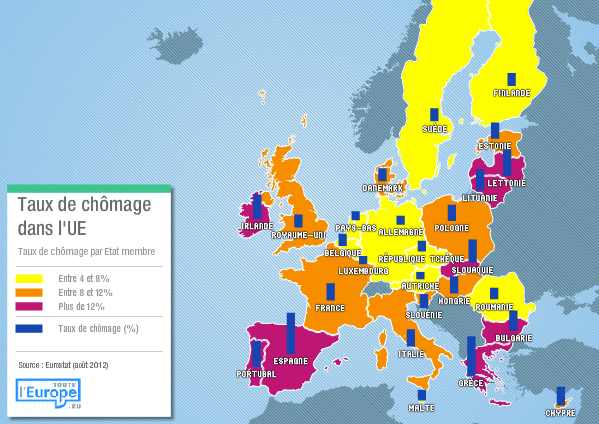
\includegraphics[width=0.98\linewidth]{../resources/illustrations/chom}
\caption{Taux de chômage dans l'UE en août 2012 \cite{chom}}
\label{chom}
\end{figure}
\begin{figure}[p]
\centering
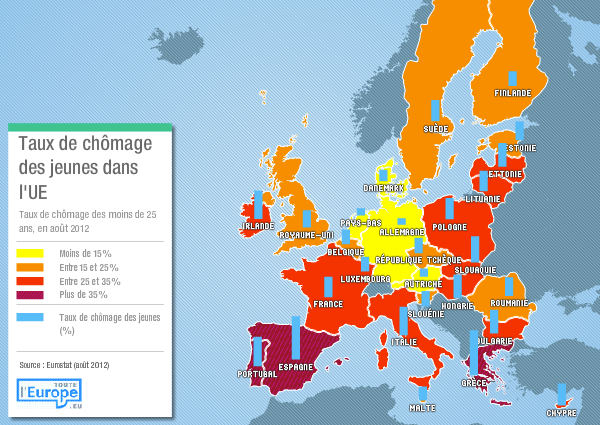
\includegraphics[width=0.98\linewidth]{../resources/illustrations/chom_jeunes}
\caption{Taux de chômage des jeunes dans l'UE en août 2012 \cite{chom_jeunes}}
\label{chom_jeunes}
\end{figure}
Commençons tout d'abord par examiner les données du chômage des jeunes comparées aux données globales du chômage (voir figures \ref{chom} et \ref{chom_jeunes}). Comme nous pouvons le constater, le chômage des jeunes est en moyenne deux fois plus important que le taux général du chômage en Europe. Cette disparité a de nombreuses explications dont certaines économiques. Nous pensons néanmoins que les causes dues à une formation inadaptée ne sont pas négligeables. 

En effet, les postes nécessitant une formation "classique" sont déjà occupés. Les machines remplacent peu à peu les emplois industriels. Les recruteurs attendent donc des jeunes qu'ils aient d'autres compétences : celles que les machines ou les seniors n'ont pas.

D'autre part, l'air du temps pousse les jeunes à devenir entrepreneurs de par le manque d'emplois salariés. Or les moyens à leur disposition ne permettent pas à la plupart d'entre eux de monter une entreprise.


\subsection{Difficulté des entreprises à recruter}
\begin{figure}[p]
\centering
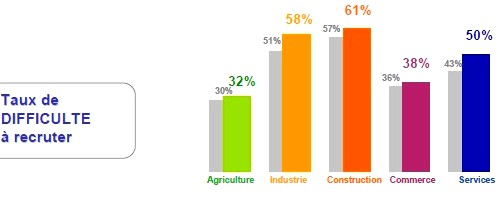
\includegraphics[trim=7cm 0cm 0cm 0cm, clip=true, scale=1]{../resources/illustrations/diff_recrut}
\caption{Taux de difficultés à recruter en 2012 en Midi-Pyrénées \cite{recrutement_midi_pyr}}
\label{diff_recrut}
\end{figure}
\begin{figure}[p]
\centering
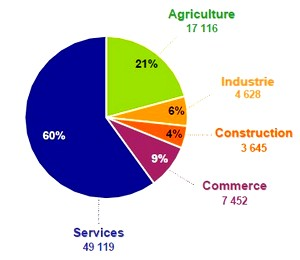
\includegraphics[scale=0.8]{../resources/illustrations/embauches}
\caption{Taux d'embauche en 2012 en Midi-Pyrénées \cite{recrutement_midi_pyr}}
\label{embauche}
\end{figure}
Des rapports de pôle-emploi indiquent clairement que malgré le taux de chômage élevé, les entreprises ont des difficultés à recruter. En effet, il n'y a pas assez de candidats et ceux-ci ne sont pas assez compétents ou pas assez diplômés. 

Comme nous pouvons le constater sur les figures \ref{diff_recrut} et \ref{embauche}, les secteurs de l'agriculture, de l'industrie et de la construction manquent de vocations (ce qui peut s'expliquer par la rigueur du travail dans ces professions). D'autre part, les secteurs des services et du commerce ont également beaucoup de difficultés à recruter et cela peut s'expliquer par l'inadéquation de la formation des candidats avec les besoins des entreprises.


\section{Les retombées imprévues de l'utilisation des technologies de la communication}
Une mauvaise utilisation des \gls{ticLabel} et plus particulièrement des réseaux sociaux conduits bien souvent à des situations dramatiques. La plupart de ces situations pourraient être évitées par le biais de préparations et de formations des jeunes à l'impact réel des réseaux virtuels.

\subsection{Des embauches influencées par internet}
De plus en plus de recruteurs (surtout aux USA) tapent le nom des candidats dans un moteur de recherche internet avant de décider de leur embauche \cite{recrutement_internet, recrut_social_network}. Ce genre de recherche permet de trouver les profils des candidats sur les réseaux sociaux (généraux ou spécialisés pour l'embauche) mais également leur site internet ou de nombreuses informations sur leur vie.

Or, si un candidat averti contrôle la diffusion des informations à son sujet sur internet, un non-averti peut diffuser des informations compromettantes pour une embauche. En effet, la publication d'un site web ou l'élaboration d'un profil sur des réseaux sociaux dédiés à l'embauche sont des points positifs ; tandis que des profils publics sur des réseaux sociaux généralistes peuvent contenir des photos, vidéos ou commentaires compromettants pour le candidat (comme des photos d'une soirées débridée ou un commentaire du candidat faisant du shopping pendant un après-midi ou il devrait être au travail par exemple).

Dans certains cas, des adolescents postent des photos et des vidéos d'eux qui les rattrapent des années plus tard lorsqu'ils deviennent adultes et cherchent un travail.

Une formation adaptée à l'utilisation des \gls{ticLabel} pourrait mener à une prise de conscience des dangers et à une responsabilisation des jeunes par rapport à ces technologies.

\subsection{Chantages, menaces et insultes sur les réseaux sociaux}
Les chantages, menaces et insultes sur les réseaux sociaux sont un des problèmes les plus importants liés à l'utilisation des \gls{ticLabel} sans formation. En effet la plupart de ces situations impliquent de jeunes adolescents qui n'ont pas conscience de la portée de leurs actes sur internet. Certains d'entre eux se déshabillent devant leur webcam, d'autres se confient à des inconnus. De ces imprudences résultent parfois des situations dramatiques comme par exemple le suicide de certains adolescents victimes de chantages ou de menaces \cite{chantage_facebook, harcel_facebook}.

Certains autres individus harcelés dans leur vie réelle voit le harcèlement se prolonger dans leur vie virtuelle. Certains autres postent des insultes sur divers réseaux sociaux sans se rendre compte de la portée de leurs actes.

Encore une fois, tous ces problèmes pourraient être aisément évités en expliquant aux enfants la portée de leurs actes sur internet.



\section{Décrochages et échecs scolaires}
Les points que nous avons abordés précédemment mettent en évidence la nécessité d'enseigner mieux les tenants et les aboutissants des \gls{ticLabel}. Ceci doit être fait en ajoutant de nouveaux enseignements aux programmes scolaires.

Cependant, d'autres problèmes liés au manque d'intégration des \gls{ticLabel} dans l'éducation émergent et ceux-ci ne sont pas réglables par l'ajout de nouveaux enseignements aux programmes scolaires. Ainsi, nous allons examiner le mal-être des élèves et des étudiants et ses manifestations : les décrochages et échecs scolaires.

\subsection{La formation des étudiants en inadéquation avec leurs attentes}


\subsection{Hyperactivité chez les gamins qui ont juste besoin d'autre chose}
% auto-formation

